\documentclass[conference]{IEEEtran}
\IEEEoverridecommandlockouts
\usepackage{cite}
\usepackage{amsmath,amssymb,amsfonts}
\usepackage{algorithmic}
\usepackage{graphicx}
\usepackage{textcomp}
\usepackage{xcolor}
\usepackage{biblatex} %Imports biblatex package
\addbibresource{reference.bib} %Import the bibliography file\
\begin{document}

\title{Enhancing Automotive Cybersecurity: Exploring Hardware Security Primitives for Resilient and Trusted Vehicle Systems }


\author{\IEEEauthorblockN{Tamal Sutradhar Rudra}
\IEEEauthorblockA{\textit{ID:212120005}\\
\textit{Department of Computer Science and Engineeering} \\
\textit{Notre Dame University Bangladesh)}\\
Dhaka, Bangladesh \\
tamal212120005@student.ndub.edu.bd}
\and
\IEEEauthorblockN{Tanvir Jahan Alin}
\IEEEauthorblockA{\textit{ID:212120008}\\
\textit{Department of Computer Science and Engineeering} \\
\textit{Notre Dame University Bangladesh}\\
Dhaka, Bangladesh \\
alin212120008@student.ndub.edu.bd}

}

\maketitle

\begin{abstract}
The integration of electronic systems and connectivity features in the automotive industry has propelled advancements in vehicle technology. However, this evolution has introduced new vulnerabilities, exposing vehicles to potential cyber threats. This paper explores the significance of enhancing automotive cybersecurity through the implementation of hardware security primitives. Making cars safe from attacks is a complicated subject that many researchers are studying. In this article, we'll discuss the current ways to keep vehicles secure using hardware modules and unique physical functions. 
\end{abstract}

\begin{IEEEkeywords}
Hardware Security, Cybersecurity, Cyberattack, Trusted Platform Module (TPM), Physically Unclonable Functions (PUFs)
\end{IEEEkeywords}

\section{Introduction}
In recent years, the automotive industry has witnessed a rapid increase in the integration of electronic systems and connectivity features in vehicles. While this trend has brought numerous benefits, it has also exposed vehicles to new cybersecurity risks. As vehicles become more connected, they become vulnerable to cyberattacks, which can have severe consequences on both driver safety and privacy. Therefore, it is crucial to enhance automotive cybersecurity to ensure resilient and trusted vehicle systems.

\section{Hardware Security Primitives}
One auspicious approach to enhance automotive cybersecurity is the use of hardware security primitives. Hardware security primitives are physical components or features integrated into the vehicle's hardware design to provide additional layers of security. These primitives can help prevent, detect, and mitigate cyberattacks by safeguarding critical vehicle functions and data.
\subsection{HARDWARE MODULES}
Hardware Module is a one kind of physical device that is used for extra security to secure the sensitive data. Mainly, it generate cryptographic key to authentication, encrypt or decrypt any kind of application or database. \par
Securing the generated keys are also a challenge for the system. The keys generated by the modules cannot be predicted by any kind of application or AI(Artificial Intelligence). It strictly has to be unique and random. The copy of the key generated by the module must be stored in secured storage so that it can be used if the key is compromised. After the key has been used the key should be permanently destroyed.\par
Researchers from the E-Safety Vehicle Intrusion
Protected Applications (EVITA) project put forward a vehicular hardware security module .\cite{wolf2012design}
Their module is a cryptographic co-processor, that is designed to be connected on vehicular communication and it comes with three different variation- "full", "medium", "light". The full version has everything to secure vehicular communication. The "medium" version has the security on inter-vehicular communication. And the "light" version only secure the interactions between ECUs and the sensors and actuators.This design has subsequently served as a source of inspiration for more recent implementations of vehicular Hardware Security Modules (HSMs). 
\subsection{Trusted Platform Module(TPM)}
Trusted platform modules (TPM) are cryptographic co-processors specifically created to embed security within larger computer systems. TPMs are permanently integrated into the system and cannot be removed. The TPM specification was initially intended for general-purpose computer systems. However, incorporating TPMs directly into vehicles poses challenges because of the limited computational resources and real-time demands specific to automotive environments. As an alternative, researchers have taken inspiration from the TPM specification to create hardware security modules (HSMs) tailored for vehicles. These vehicle-specific HSMs are designed for seamless integration into automotive systems and typically include a subset of the cryptographic components found in traditional TPMs.
\begin{figure}[htbp]
\centerline{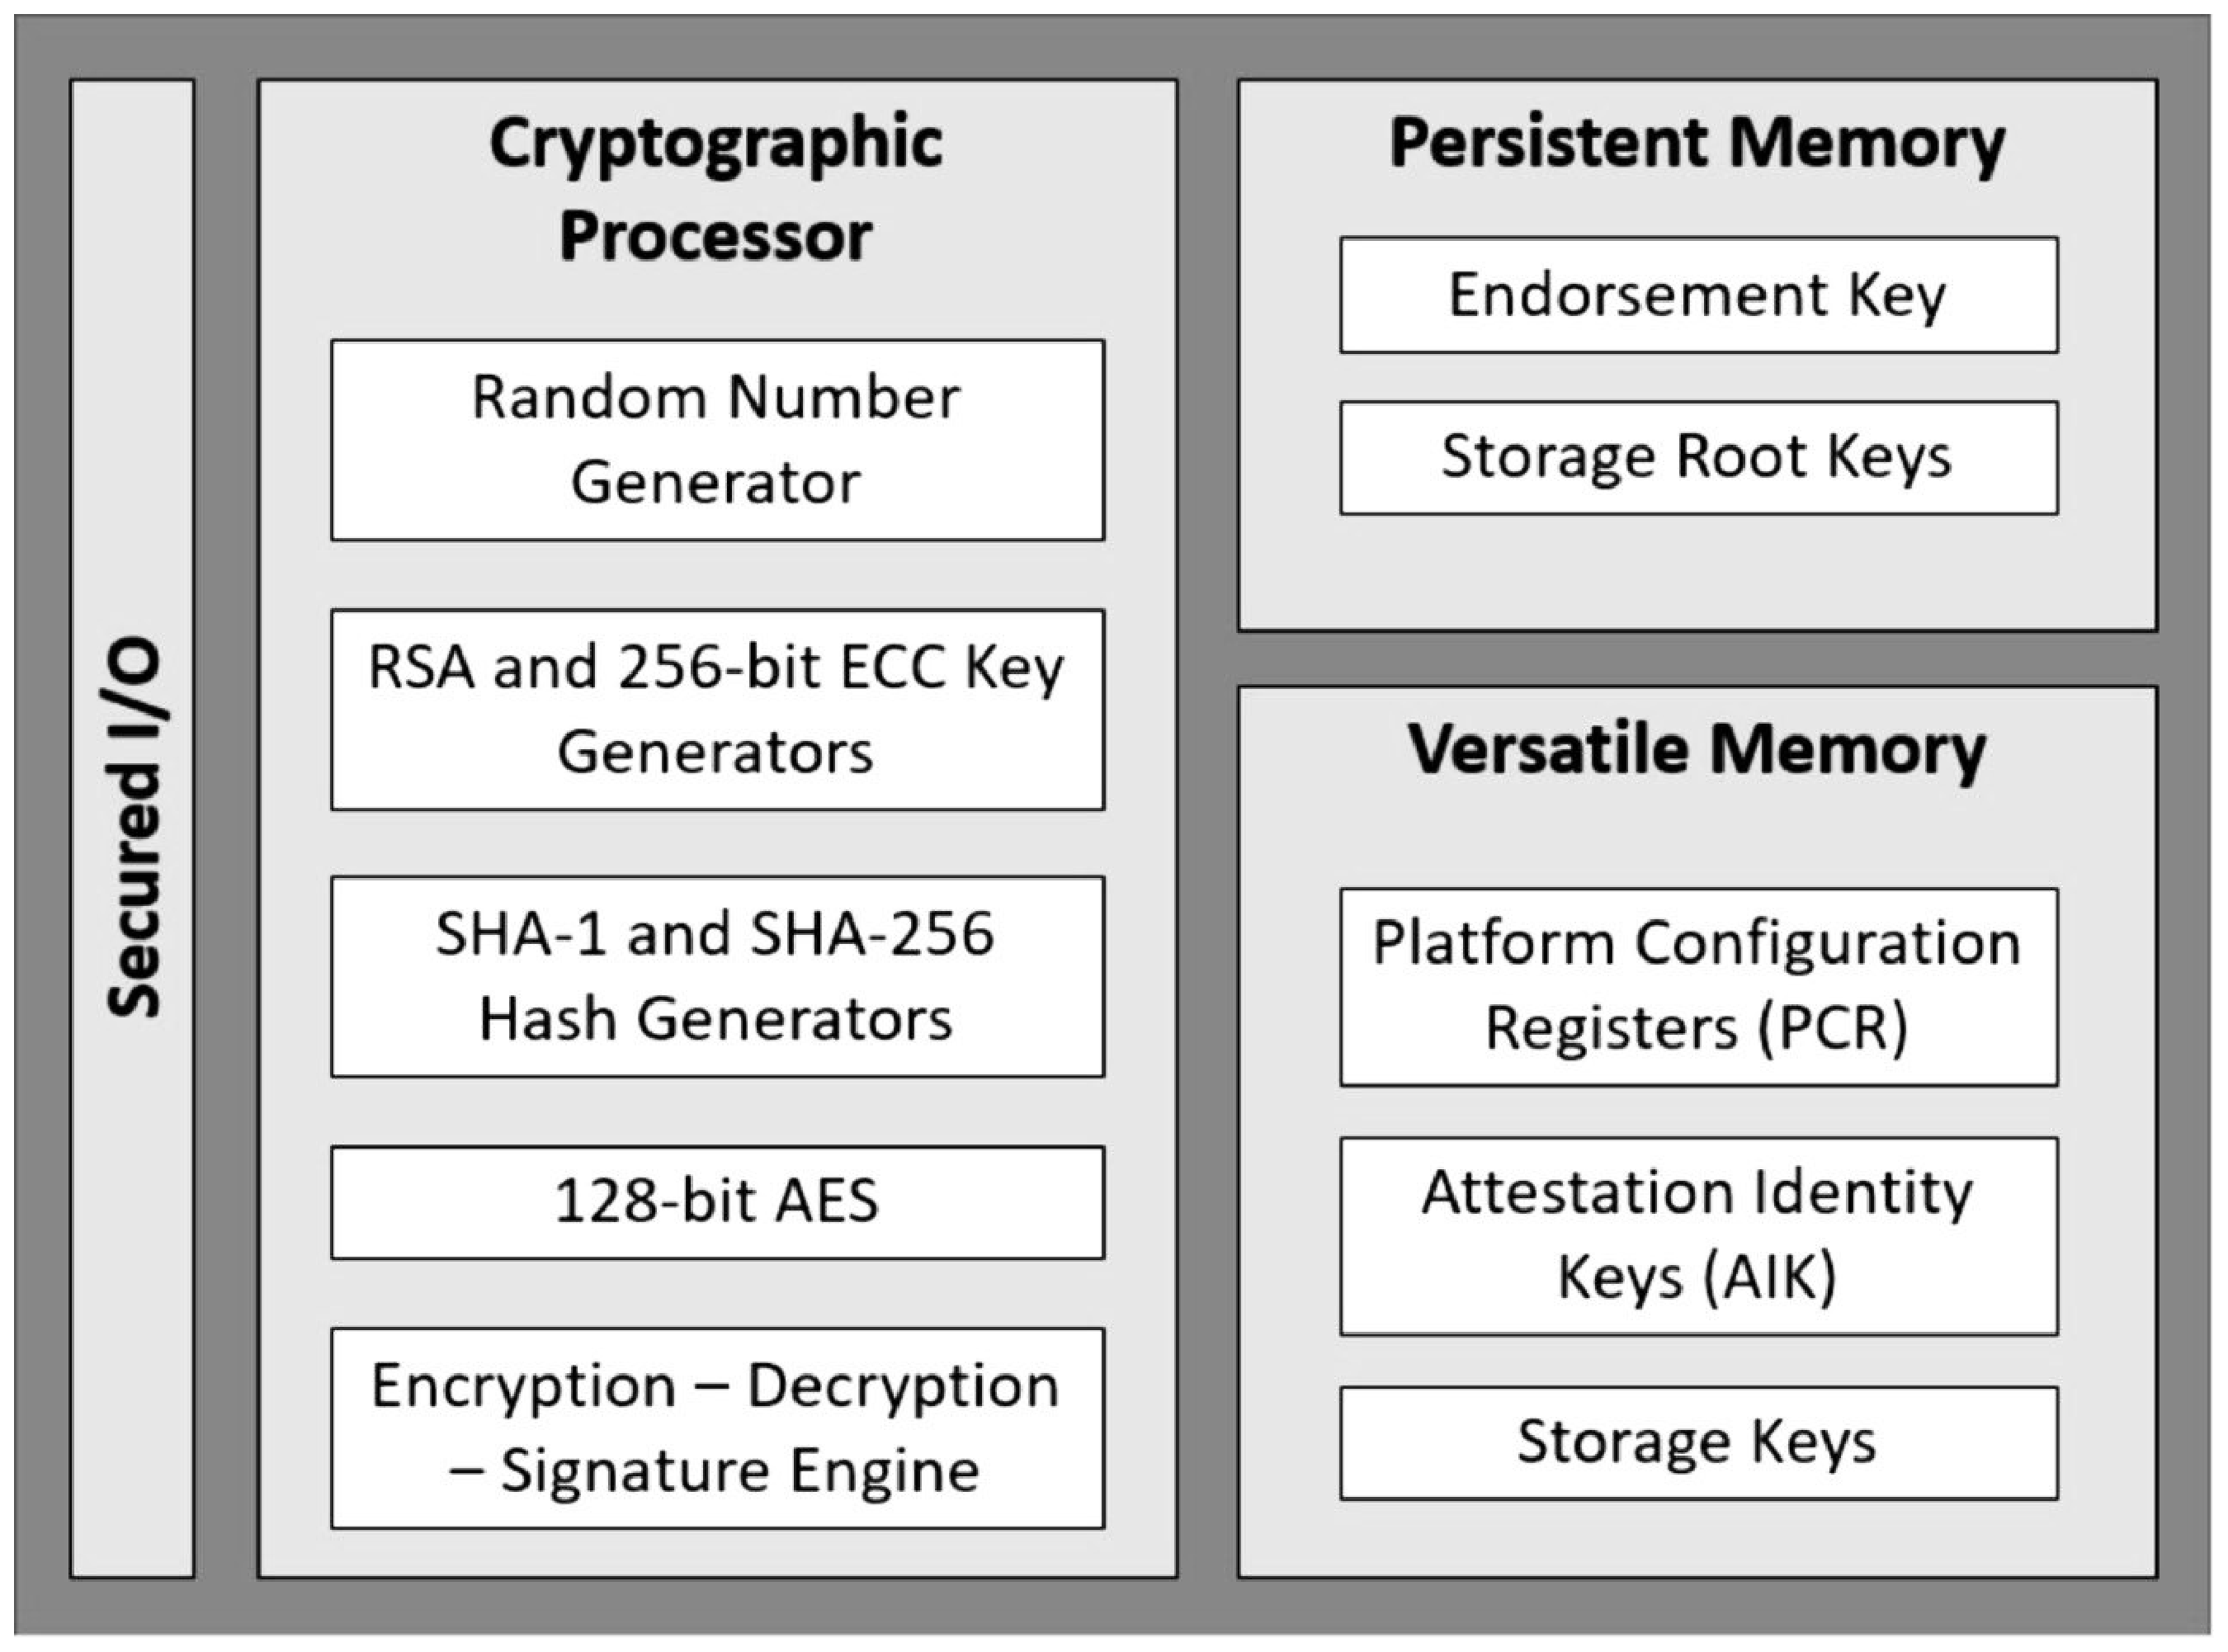
\includegraphics[width=0.5\textwidth]{TPM.eps}}
\caption{Necessary Elements of TPM 2.0}
\label{fig}
\end{figure}
\subsection{Physically Unclonable Functions}
Physical unclonable functions (PUFs) can be likened to a kind of hash function, where a particular input produces a unique output. Within PUFs, the inputs are referred to as 'challenges,' and the outputs are termed 'responses. '\cite{labrado2019hardware}
Together, a challenge and its corresponding reply are referred to as a challenge-response pair (CRP). A physically unclonable function (PUF) is considered robust when it has a significant quantity of CRPs. In an ideal scenario, it would have an exponential number of CRPs so that an n-bit strong PUF would have 2n CRPs. On the other hand , a weak PUF has a very limited number of CRPs (typically just one).\cite{oriero2019survey}

\section{PUFs for Security in Vehicles }
Physically unclonable functions (PUFs) offer a range of possible applications in automotive security and can be custom-designed for integration into these systems. \cite{labrado2018design}
The special qualities inherent to PUFs make them suitable for applications that would be unfeasible using traditional technology. This section will point out some of the possible security uses of PUFs, including storing keys, creating pseudonyms, and enabling vehicle-to-vehicle communication. 
\begin{figure}[htbp]
\centerline{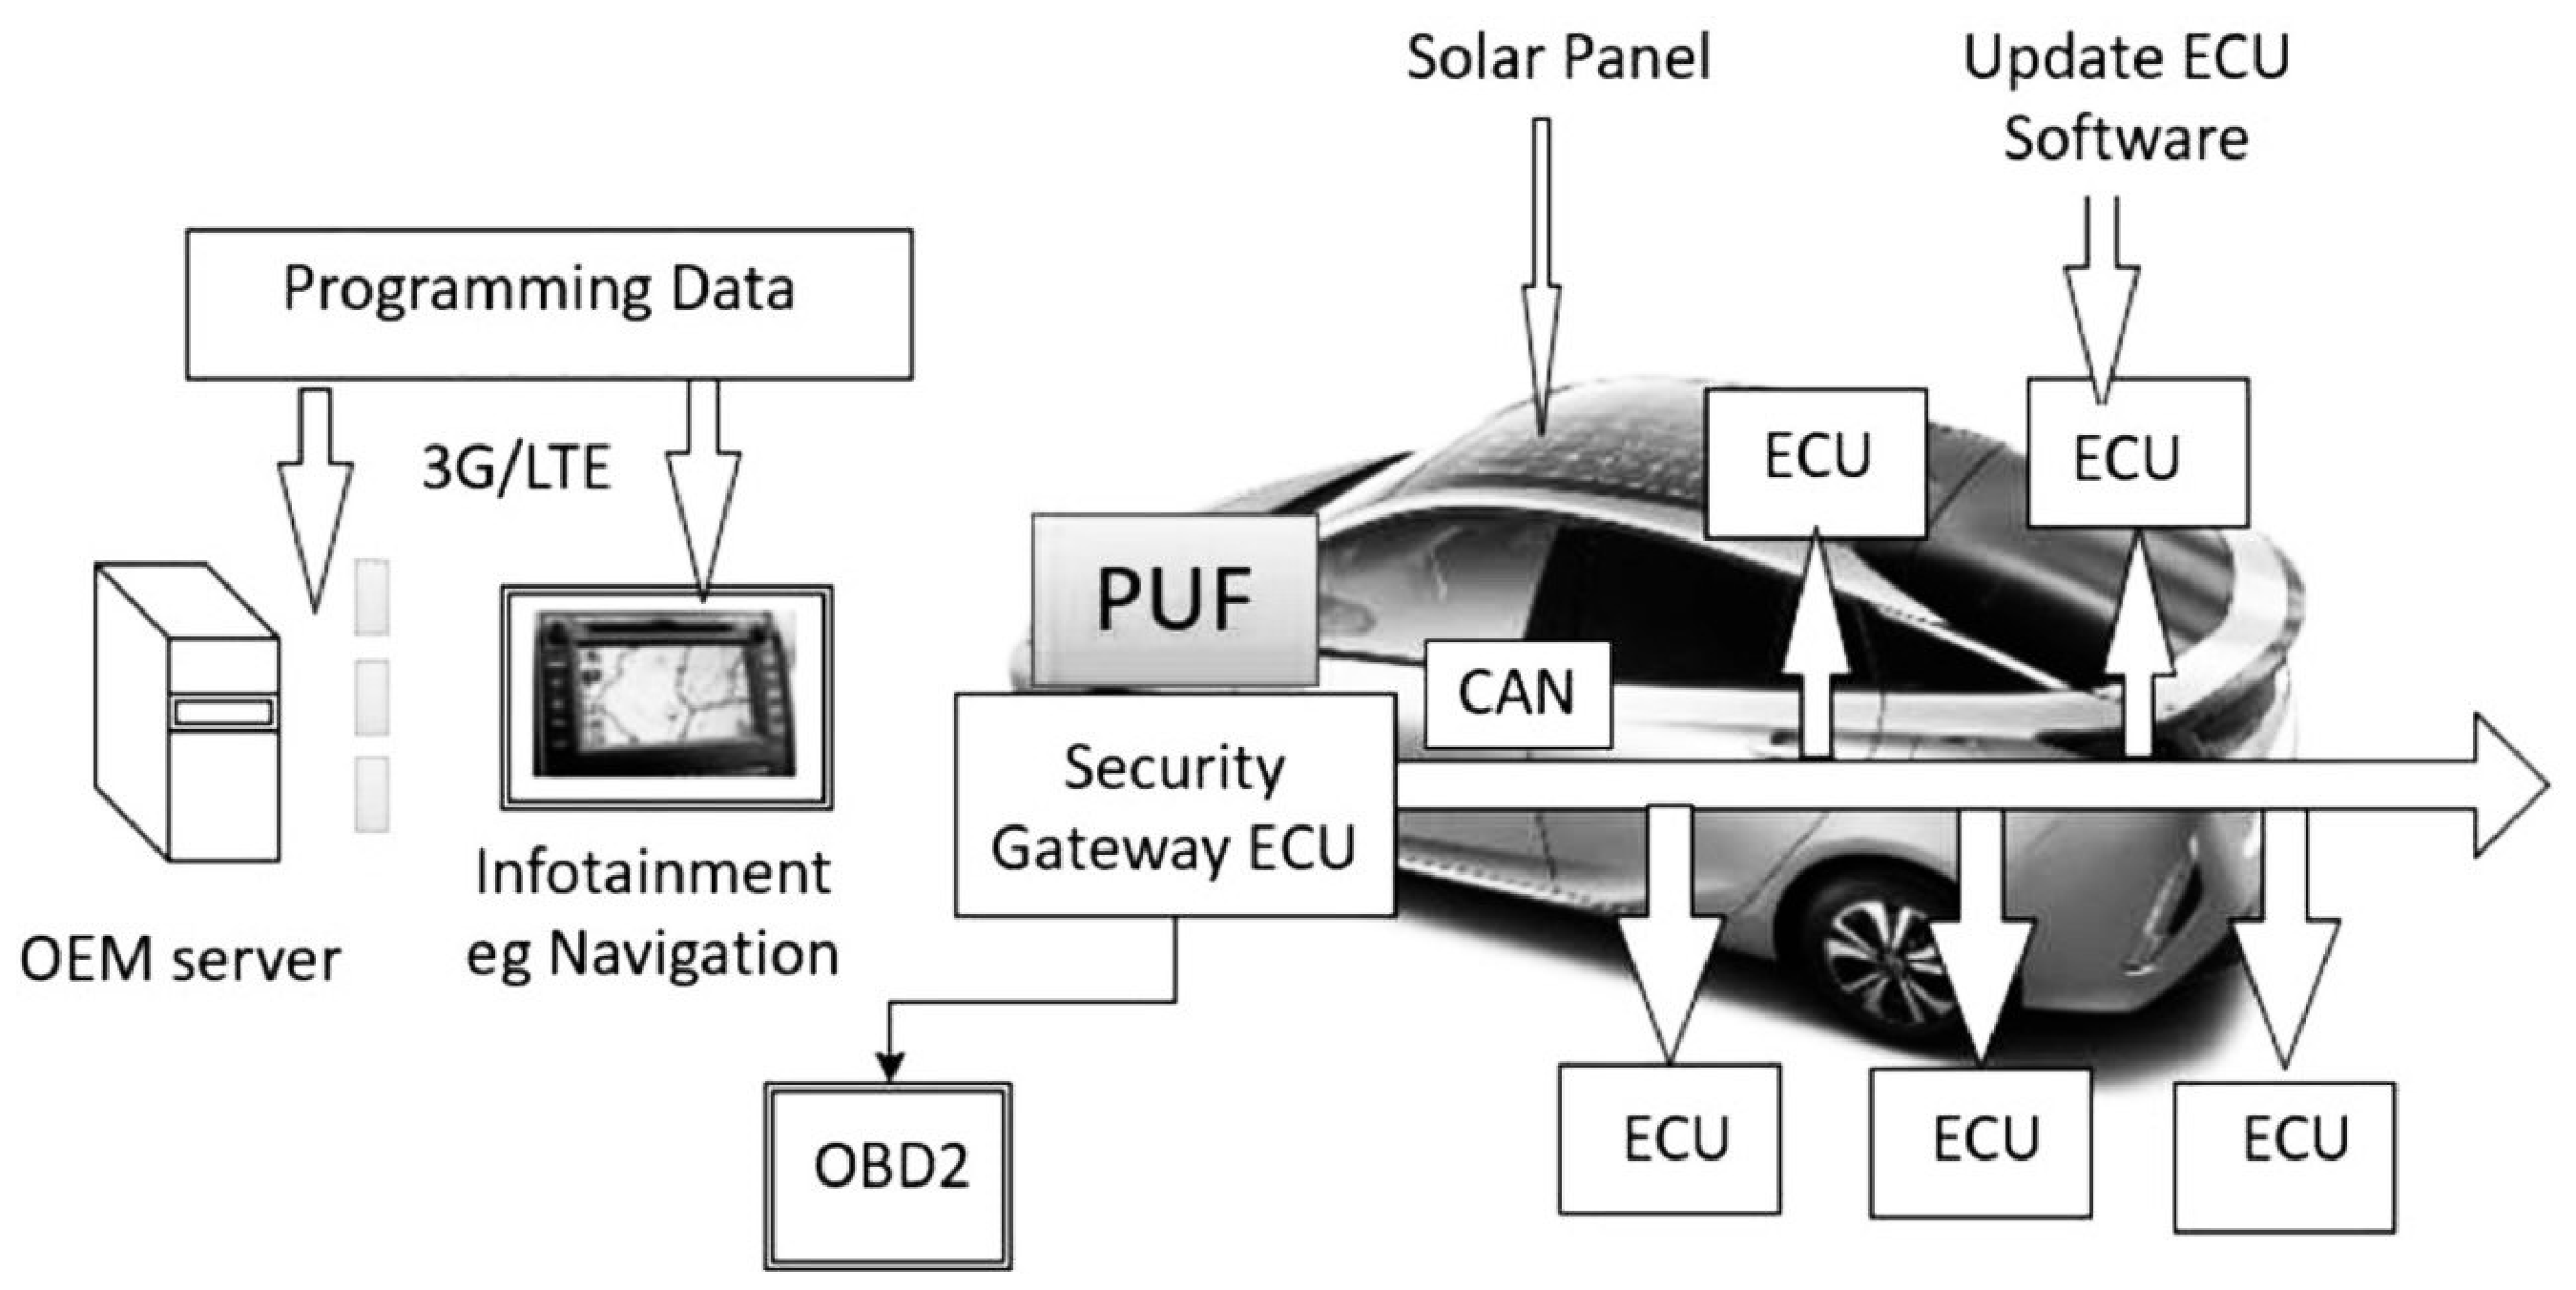
\includegraphics[width=0.5\textwidth]{PUF.eps}}
\caption{Incorporation of PUF technology to ensure the security of software updates in the automotive industry.\cite{hiroyuki2015puft}}
\label{fig}
\end{figure}
\subsection{Using PUF for Safe Data Storage}
 Scientists have suggested the utilization of physically unclonable functions (PUFs) as a means to store private keys for use in vehicle communication. \cite{feiri2013efficient}
 Conventional key storage techniques usually rely on secure memory. However, their approach enables the safe storage of keys in memory that isn't inherently secure. This is accomplished by generating keys based on the responses of a physically unclonable function (PUF), which guarantees that an attacker would need to have the physical device itself to retrieve the key. \cite{labrado2019hardware}
 The suggested techniques include the use of either a strong PUF or a weak PUF. \cite{feiri2013efficient}
 \par In the article written by Petit and colleagues, they suggest a different way to store data. \cite{petit2012potential}
 In this approach, the unique response generated by the PUF is employed to create a pseudonym consisting of a public key and a private key pair. A central Certificate Authority (CA) issues a certificate as evidence that it has confirmed the legitimacy of this pseudonym. This certificate can be included in communications with an outside entity. \cite{labrado2019hardware}
\subsection{ Using PUF for Communication Between Vehicles }
Scientists have suggested using PUFs as a component in a bigger communication system that can prevent attacks from groups of adversaries. \cite{dolev2015optical}
In this scenario, a vehicle communicates with nearby vehicles. To ensure the right vehicles receive these messages, sensors are used to visually connect each message with the correct vehicle. This visual connection helps the vehicle determine where the other vehicles are located relative to itself. This information is useful for responding to warning messages from those vehicles.\par

\begin{enumerate}
    \item PUF in inter-vehicular Communication:
Scientists have suggested a method for incorporating Physically Unclonable Functions (PUFs) into a broader communication system with the capability to thwart coalition attacks by adversaries.\cite{dolev2015optical}
In a coalition attack, multiple adversaries mimic the sender and recipient by intercepting and subsequently relaying messages to their intended targets. In the described scenario, a specific vehicle is engaged in communication with other nearby vehicles. To ensure the legitimacy of these communications, sensors are used to visually link each message to the correct vehicle, providing a relative location understanding of the communicating vehicles. This knowledge can be valuable for the receiving vehicle in responding to warning messages from its counterparts.\par
    \item Incorporating PUF with ECU:
The researchers propose a method to stop Denial of Service (DoS) attacks on the CAN bus by introducing the capability to verify the identity of connected ECUs.\cite{aishwarya2016authentication}
The suggested approach involves the allocation of a unique identifier (ID) to every Electronic Control Unit (ECU) connected to the CAN bus. Each ID is linked to specific challenge-response pairs (CRPs) generated by Physical Unclonable Functions (PUFs) integrated into each ECU. A centralized reference monitor (RM) securely stores copies of these IDs and CRPs for all ECUs within a trusted platform module (TPM). This data is established and loaded during the vehicle's assembly process. To initiate communication on the CAN bus, any ECU must undergo authentication by the RM.

A similar strategy, as proposed in, employs PUFs within individual ECUs to create private/public key pairs for each ECU and a central server.\cite{han2018bad} These key pairs are initially used to register each ECU's ID with the server. Subsequently, the server authenticates communication sessions between ECUs.\cite{labrado2019hardware1}

\end{enumerate}

However, adversaries, even if they merely forward intercepted messages without altering them, can deceive targeted vehicles into visually associating with the adversary instead of the actual intended recipient. This deceptive practice can pose risks, particularly when vehicles are responding to emergency warnings like sudden braking.\par

To mitigate these issues, the researchers propose the development of a message authentication method that is non-forwardable, rendering it immune to coalition attacks. Vehicles are issued certificates by a trusted Certificate Authority (CA), containing physical characteristics for vehicle identification and challenge-response pairs (CRPs). When a vehicle seeks to initiate communication, it shares its certificate with the intended recipient. The recipient processes the information from the certificate and configures a laser based on the challenge parameters within the certificate. The recipient's laser stimulates the optical Physical Unclonable Function (PUF) on the sending vehicle and records the response. If the recorded response aligns with the response in the certificate, the receiving vehicle authenticates the sender. This process is then reversed, with roles swapped, allowing the sending vehicle to authenticate the receiving vehicle.\par

However, there's a potential issue. Adversaries can forward messages, making the targeted vehicles mistakenly connect to the adversary instead of the intended recipient. Even if adversaries simply forward messages without altering them, the attacked vehicle may wrongly identify the adversary as the intended communication partner. This could be dangerous, especially when the attacked vehicles need to respond to emergency warnings, like sudden braking maneuvers.
\section{Discussion and Final Thoughts  }
Even the fundamental building blocks of hardware security, such as TPMs, HSMs, and PUFs, can have their own security weaknesses due to design flaws.Recently, scientists uncovered two ways to breach TPMs by exploiting new design flaws that can be fixed with firmware updates. \cite{han2018bad}Furthermore, numerous widely used cryptographic algorithms, like RSA, in TPMs and HSMs, can be exploited by quantum attacks. \cite{chen2016report}
Machine learning-based modeling attacks have been demonstrated to compromise the security of multiple PUFs.\cite{delvaux2019machine}These weaknesses introduce further complexities in design but are not insurmountable obstacles. The elements examined in this study offer a strong basis for the creation of security systems for vehicles.\cite{labrado2019hardware1}


\section{Conclusion}
In conclusion, the exploration of hardware security primitives as a means to enhance automotive cybersecurity presents a promising path towards building resilient and trusted vehicle systems in today's increasingly connected automotive landscape. The adoption of security measures such as Secure Boot, Trusted Execution Environment (TEE), and hardware encryption offers tangible benefits in safeguarding critical vehicle functions and data from cyber threats.\par

By implementing these hardware security features, automakers can provide a safer and more secure driving experience for consumers. Resilient systems capable of detecting and recovering from cyberattacks minimize the potential disruptions to vehicle functionality. Concurrently, trusted systems foster a strong sense of confidence in the security and privacy of the vehicle, bolstering the trust between drivers and their automobiles.\par

As the automotive industry continues to evolve, it is imperative to prioritize and invest in robust cybersecurity measures to address the evolving threats. Hardware security primitives play an indispensable role in this endeavor, ensuring that vehicles remain at the forefront of innovation while preserving the safety and privacy of their occupants. In doing so, the industry can move forward with the assurance that automotive cybersecurity remains a top priority in the ever-connected and technology-driven world of automobiles.

\printbibliography %Prints bibliography

\end{document}
